% !TEX root = main.tex
\begin{figure} 
    \centering
  \subfloat[QPSK \label{1a}]{%
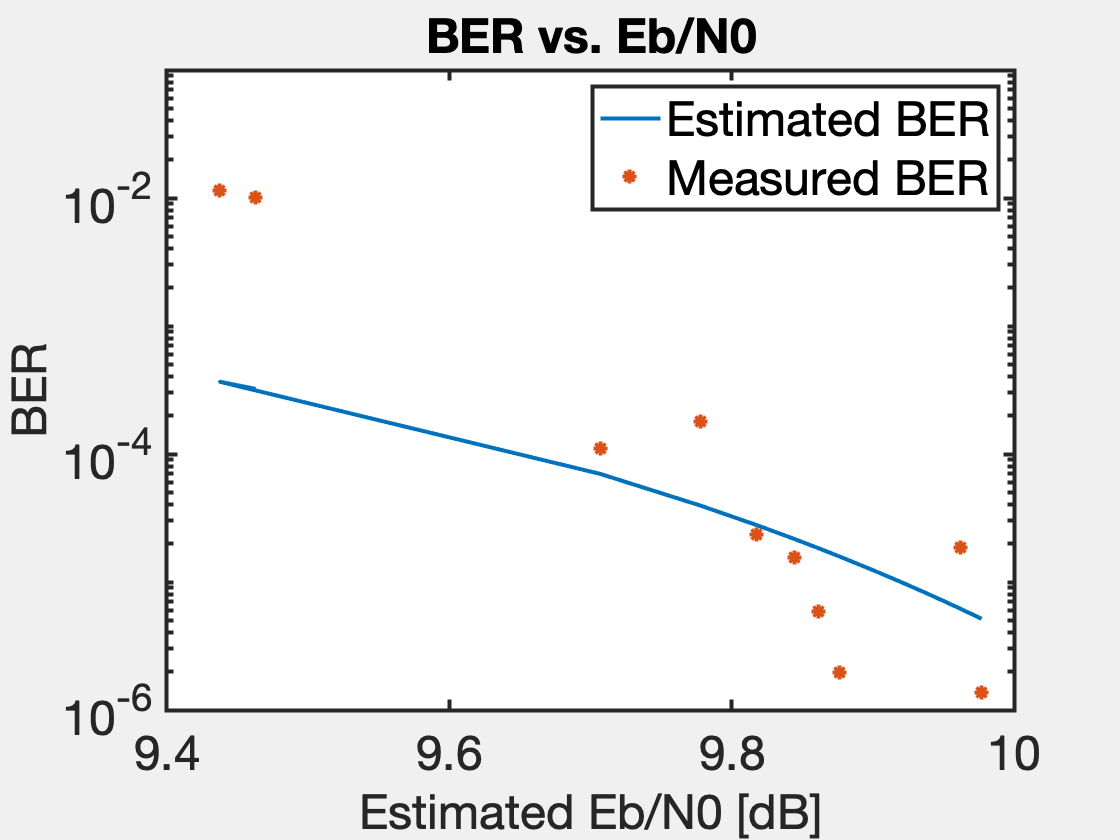
\includegraphics[width=0.45\linewidth]{BERvsSNRQPSK.png}
}
  \subfloat[QAM-16\label{1b}]{%
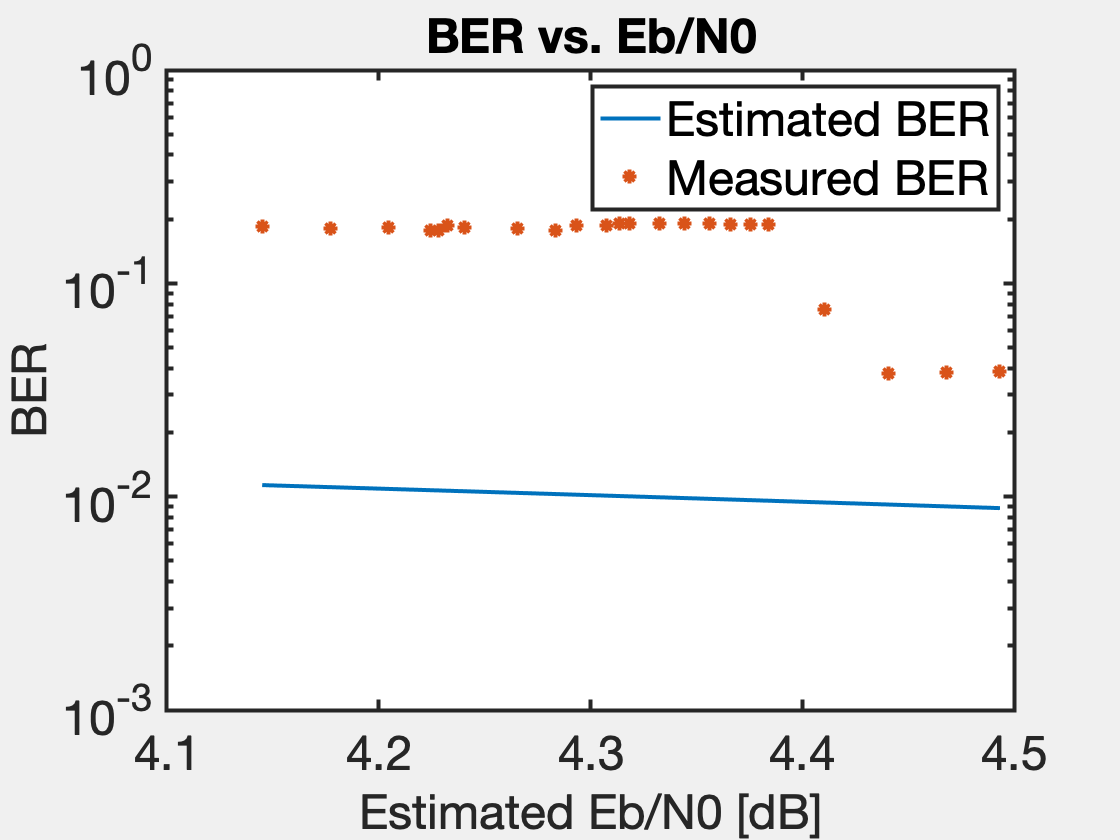
\includegraphics[width=0.45\linewidth]{BERvsSNRQAM.png}

}
  \caption{BER vs. SNR for both modulation formats. The estimated BER is the theoretical BER based on the estimated values for \ebnot and true BER is the actual calculated BER}
  \label{fig:ber_vs_snr} 
\end{figure}